\documentclass[border=10pt]{standalone}
\usepackage{tikz}

%Provide default strings for packet field descriptions in english if anything else not set

\providecommand{\ADDRSTR}{Address}
\providecommand{\SIZESTR}{Size}
\providecommand{\TERMSTR}{Terminator}
\providecommand{\DATASTR}{Data}

\usetikzlibrary{positioning,arrows,decorations.pathreplacing}

\begin{document}
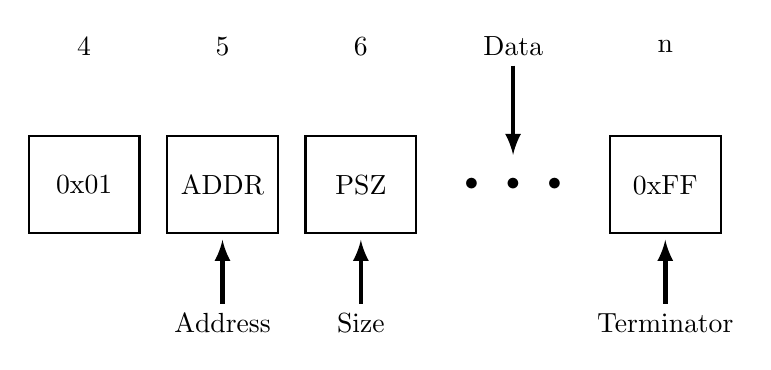
\begin{tikzpicture}[node distance=50pt,minimum size=1pt,auto]

\tikzstyle{pfield}=[rectangle,minimum width=40pt,minimum height=35pt,draw=black,thick];

\node [pfield] (b0) {0x01};
\node [pfield] (b1) [right of=b0] {ADDR};
\node [pfield] (b2) [right of=b1] {PSZ};
%\node [pfield] (b3) [right of=b2] {ADDR};
%\node [pfield] (b4) [right of=b3] {PSZ};

\node  (d0) [right of=b2,xshift=-10pt] {$\bullet$};
\node  (d1) [right of=d0,xshift=-35pt] {$\bullet$};
\node  (d2) [right of=d1,xshift=-35pt] {$\bullet$};

\node [pfield] (b5) [right of=d2,xshift=-10pt] {0xFF};

%\draw [decorate,decoration={brace,amplitude=10pt,raise=5pt}] (b1.315) -- (b0.225) node [black,midway,align=center,yshift=-15pt] {\SDSTR};

%\draw [decorate,decoration={brace,amplitude=10pt,raise=5pt}] (b3.315) -- (b2.225) node (t0) [black,midway,align=center,yshift=-15pt] {\TDSTR};

%\node (t1) at (t0 -| b4) {\CMDSTR};

\node (t1) [above of=d1] {\DATASTR};
\node (t2) [below of=b1] {\ADDRSTR};
\node (t3) at (t2 -| b2) {\SIZESTR};

\node [align=center] (t4) at (t2 -| b5) {\TERMSTR};

\path [-latex,ultra thick, shorten >=5pt] (t1) edge (d1);
\path [-latex,ultra thick, shorten >=2pt] (t4) edge (b5);
\path [-latex,ultra thick, shorten >=2pt] (t3) edge (b2);
\path [-latex,ultra thick, shorten >=2pt] (t2) edge (b1);

%field number
\node [above of=b0] {4};
\node [above of=b1] {5};
\node [above of=b2] {6};
%\node [above of=b3] {N};
%\node [above of=b4] {6};
\node [above of=b5] {n};

\end{tikzpicture}
\end{document}